 \chapter{Soliton Crystals} \label{ch:SolitonCrystals}

This chapter presents results on the self-organization of ensembles of soliton in optical microring resonators. The reported phenomenon explains physics that goes beyond the basic LLE model of Kerr-comb formation, as is described in Sec. \ref{sec:crystallizationmechanism}. We refer to these self-organized ensembles as `soliton crystals,' which extends an analogy to condensed-matter physics that has been made in other nonlinear-optical systems, including single-pass nonlinear fiber systems \cite{Zajnulina2017} and harmonically mode-locked fiber laser \cite{Haboucha2008,Amrani2011a}, where a mechanism for soliton crystallization that is based on two distinct timescales of the laser medium \cite{Haboucha2008c} and is different from the one presented here was identified. Notably, the spatiotemporal chaos exhibited in the LLE was referred to as a `soliton gas' in early studies of nonlinear dynamics in passive fiber-loop resonators \cite{Malomed1998,Mitschke1998,Schwache1997}. 

Soliton crystals are soliton ensembles in which each soliton lies on a lattice site $\theta_n= 2\pi n/N$ in the co-moving frame, where $N$ is the lattice parameter that arises from the fundamental physics of the system as described below and $n$ indexes over the lattice sites. We have observed a wide variety of crystal configurations, and we present some of them in Sec. \ref{sec:crystallography}; typically a small fraction of lattice sites are occupied by solitons. Soliton crystals are characterized by stable, dense occupation of the resonator by soliton pulses, and this dense occupation comes with high circulating power relative to single solitons or few-soliton ensembles. This important fact allows soliton crystals to be generated with decreasing pump-laser frequency scans across the resonance that are adiabatic in the sense that both the resonator temperature and the intracavity waveform are maintained at the values\footnote{\color{red}something about chaos\color{black}} that would be expected from the instantaneous $\alpha$ and $F^2$ parameters throughout the scan.

We demonstrate generation of a soliton crystal in Fig. \ref{fig:SCexample}; it is useful to contrast this with the behavior exhibited in Fig. \ref{fig:solitonsteps}. 

\begin{figure}[htpb]
	\begin{center}
		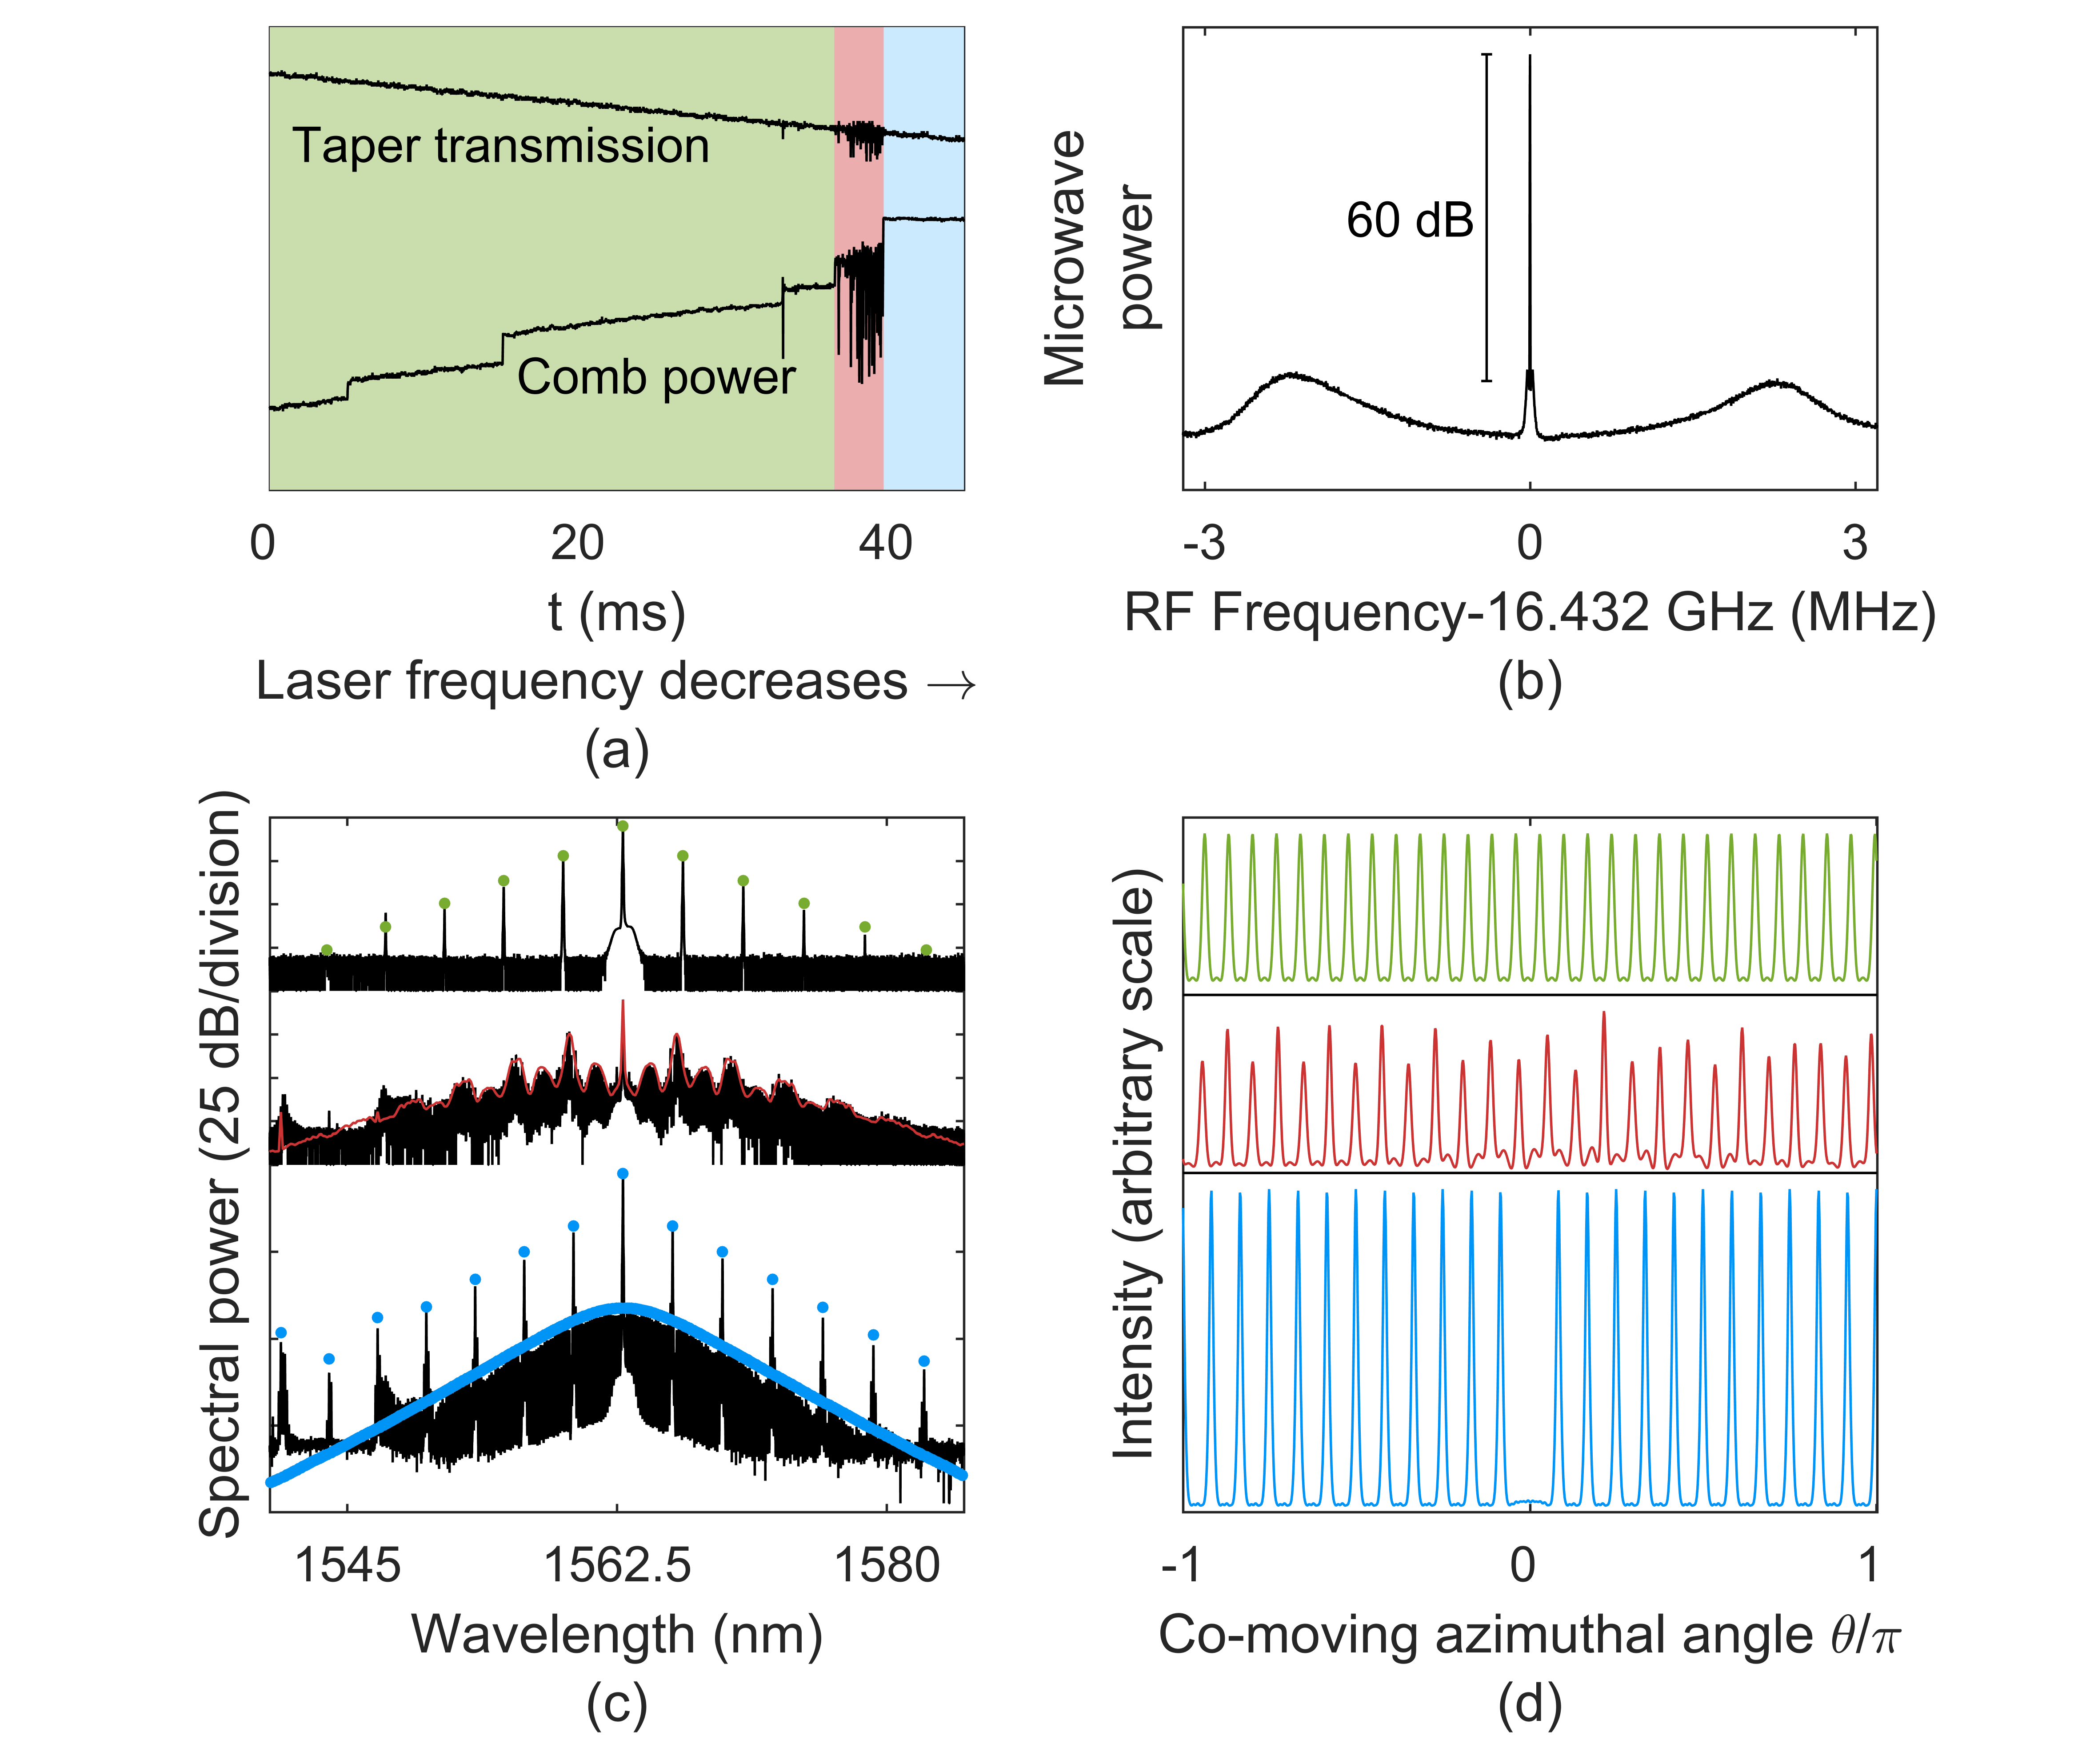
\includegraphics{\FigPath/Figures/SolitonCrystals/SCexample.png}
	\end{center}
	\caption[Figure Title]{\textbf{title}text}
	\label{fig:SCexample}
\end{figure} 

\section{Mechanism of soliton crystallization}

Fig. \ref{fig:SCexample} presents the optical spectrum and corresponding time-domain simulation of a soliton crystal. This spectrum consists of widely-spaced primary-comb lines that are separated by many resonator FSR, superposed on top of an underlying $\mathrm{sech}^2$ spectrum of the kind that corresponds to a single soliton. In fact, this spectrum can be understood through the basic superposition principle of the electric field: The primary comb spectrum with spacing $N\times f_{FSR}$ corresponds to a train of $N$ uniformly spaced pulses in the resonator. The observed crystal spectrum corresponds to such a pulse train with a single vacancy, where a pulse is missing. The effect of this vacancy on the spectrum can be understood by considering the addition of an \textit{out-of-phase} pulse to the pulse train that coincides in time with one of the existing pulses---in the time domain this corresponds to removal of one of the pulses, while in the spectral domain this corresponds to the addition (in the phase-sensitive field quantity) of the primary-comb spectrum and the single, out-of-phase soliton. 

The simulated time-domain waveform of the soliton crystal presented in Fig. \ref{fig:crystal1} is not stable in evolution under the LLE. The observed width of the spectrum fixes the ratio between $\alpha$ and $\beta$, as seen from Eq. \ref{eq:LLEsoliton}. This ratio then fixes the temporal duration of the solitons, in turn determining the characteristic length of their interactions. When an attempt to simulate the crystal according to the LLE is made with parameters $\alpha=??$ and $\beta=??$ that give agreement with the measured width of the optical spectrum, it is found that pair-wise attractive interactions between solitons lead to collapse of the crystal.

A stabilization mechanism that goes beyond the physics of the LLE is responsible for the stability of this and other soliton crystals. The stabilization mechanism arises from avoided mode-crossings in the resonator spectrum. A `mode family' corresponds to a set of circulating modes that have different azimuthal mode numbers but (approximately, neglecting wavelength-dependent effects) the same transverse spatial mode profile. As discussed in Sec. \ref{something}, some resonators support multiple mode families, each with its own free spectral range at a given wavelength. Although the modes in different families are in principle orthogonal, coupling between them can be provided, for example, by the coupling waveguide or tapered fiber used to drive the resonator. If a coupling exists between two modes that are sufficiently close in frequency, the frequencies of the modes become displaced from their frequencies in the absence of this coupling \cite{Haus1991}. This affects Kerr-comb generation in the affected mode families, because the local detuning between the resonator modes and the Kerr-comb modes is changed as a result of the mode crossing. This comb-resonator detuning change may either enhance or inhibit nonlinear frequency conversion to the effected Kerr-comb modes, thereby changing the amplitude of these modes in the comb spectrum. 

It has been reported that avoided mode crossings in the resonator spectrum can inhibit soliton generation in anomalous-dispersion resonators\cite{4,6}, while they can facilitate the formation of Kerr-combs in normal-dispersion resonators\cite{37} \todo{other citations here}. Here we are interested specifically in the impact of the avoided mode crossing on the waveform of a soliton. For simplicity, we focus on the case where a single comb mode is affected by the mode crossing. When the change in the comb-resonator detuning increases the amplitude of that mode in the soliton's spectrum, the change to the time-domain waveform can be understood by considering this increase as the addition of extra CW light at the frequency of that mode. This extra CW light exists throughout the cavity, and it leads the introduction of periodic intensity oscillations in the background on which the soliton rides as the new CW light beats against the existing background at the pump frequency. This new background wave in the cavity has a period of $2\pi/\mu_\times$ in the angular coordinate $\theta$, where $\mu_\times$ is the pump-referenced mode number of the Kerr-comb mode affected by the mode crossing, for which the detuning has been shifted. 

When several of these perturbed solitons co-propagate in a resonator, they interact through their extended waves and arrange themselves such that the waves constructively interfere. Each soliton then lies at the peak of a single extended background wave in the resonator, similar to predictions for bichromatically pumped Kerr combs\cite{38}. Importantly, temporal separations between solitons are therefore required to be multiples of this wave's period, and the wave stabilizes the crystal against the attractive interactions discussed above. Furthermore, the wave's amplitude, and thus the strength of the crystal against perturbations, increases with the number of co-propagating perturbed solitons. Finally, we note that at least within the assumption of single-mode perturbation of the comb's spectrum, this interaction has infinite range. 

We note that the mechanism observed here builds on previous reports of related phenomena. It has been shown that local interactions between cavity solitons can arise through decaying oscillatory tails \cite{39}, leading to the formation of small, locally ordered soliton molecules. Furthermore, it has been shown that the injection of an additional CW laser into a passive fiber-ring resonator can result in the generation of uniform distributions of solitons \cite{40}. The mechanism we report here can be viewed as a variant of this CW-soliton interaction in which the `injected' CW laser is provided by the affect of the mode crossing on the solitons' spectra.

We connect this discussion to the soliton-crystal spectrum presented in the bottom trace of Fig. \ref{fig:SCexample}c---this spectrum exhibits excess power near pump-referenced modes numbers $\mu_{\times,1}=5\times24=120$ (1,547 nm) and $\mu_{\times,2}=7\times24=168$  (1,541 nm). Also visible is suppressed comb generation where the comb-resonator detuning has been increased. Here 24 FSR is the spacing of the prominent primary-comb lines. 

\subsection{Simulation of soliton crystals}

To incorporate the stabilization mechanism described above into numerical simulations, we incorporate into the LLE a reduced comb-resonator detuning on a single mode $\mu_\times$. The mode-dependent comb-resonator detuning can be calculated as:
\begin{align}
\alpha_\mu&=-2(\Omega_0-D_1+\omega_\mu)/\Delta\omega,\\
&=\alpha-\beta\mu^2/2.
\end{align}
Here $\Omega_0$ is the frequency of the pump laser, $\omega_\mu$ is the set of cavity resonance frequencies referenced to the pumped mode, and $D_1=\partial\omega_\mu/\partial\mu|_{\mu=0}$ is the resonator's FSR at the pumped mode and is also assumed to be the Kerr-comb's repetition rate. The dispersion operator is applied in the frequency domain in numerical simulations of the LLE (see \ref{app:numericalsims}), which facilitates inclusion of $\delta$-function perturbations to the comb-resonator detuning as:
\begin{equation}
\alpha_\mu=\alpha-\beta\mu^2/2+\Delta\alpha_\mu,
\end{equation}
where
\begin{equation}
\Delta\alpha_\mu=2(\omega_\mu-\omega_{\mu,0})/\Delta\omega
\end{equation}
is the normalized change in the frequency of mode $\mu$ from the expected frequency $\omega_{\mu,0}$. 

We demonstrate the stabilization mechanism and the simulation method by presenting a simulation of the crystal in Fig. \ref{fig:SCexample}c. The simulation is shown in Fig. \ref{SCexampleSim}. This figure illustrates that, without the stabilization mechanism, the crystal will collapse. We note that a phenomenological application of coupled-mode theory\cite{Haus1991} could be used to calculate the full perturbation to the soliton spectrum by the mode crossing, but we find that to explain the existence of this 23-soliton crystal and the apparently exact circumferential spacing of the pulses by $2\pi/24$ radians, it is sufficient to incorporate into the LLE a reduced comb–resonator detuning on only mode 120 or on mode 168, where the excess power is largest. The crystal is then a steady-state solution of the resulting perturbed LLE.

\begin{figure}[htpb]
	\begin{center}
		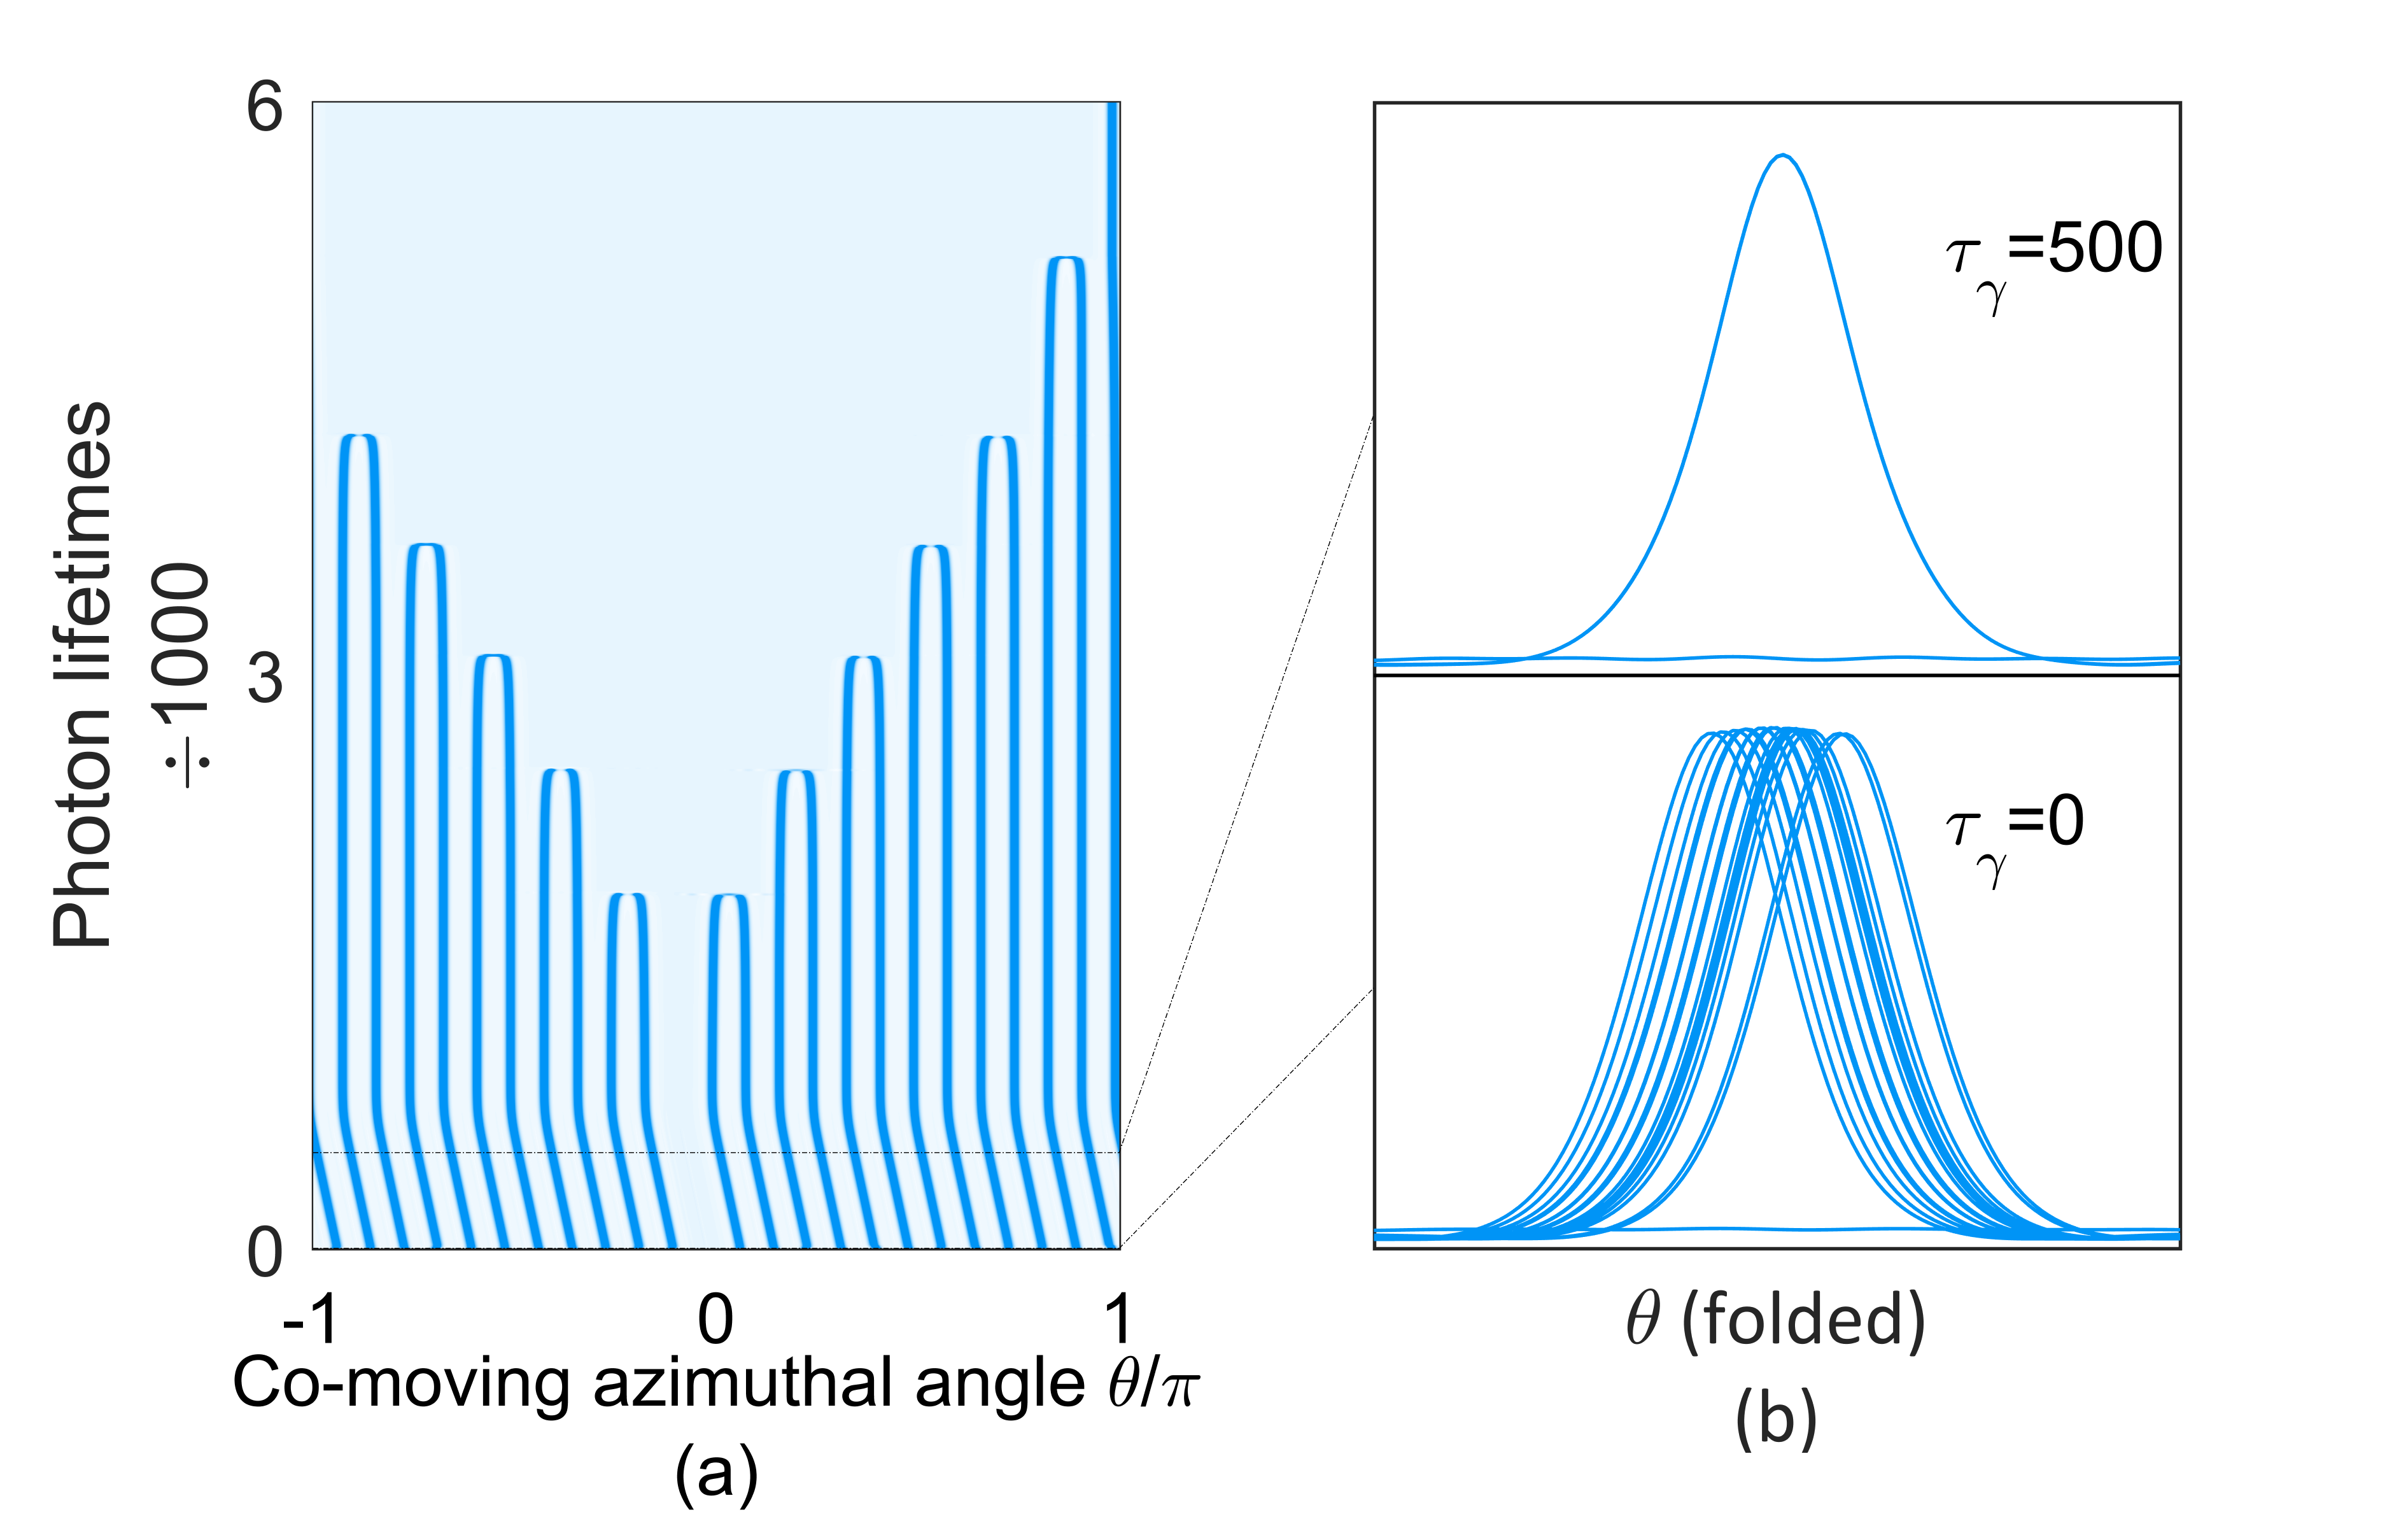
\includegraphics{\FigPath/Figures/SolitonCrystals/SCexamplesim.png}
	\end{center}
	\caption[Figure Title]{\textbf{title}text}
	\label{fig:SCexamplesim}
\end{figure} 


\section{Case study: superstructured crystal}

We consider a second specific example of a soliton crystal. The measured optical spectrum for this crystal is shown in Fig. \ref{fig:SCsuperstructure}a. This crystal exhibits superstructure---the soliton pulse train isnearly periodic in a small unit cell but is modulated with a larger periodicity. This rseults from the frustrated uniform distribution of 16 solitons with allowed inter-soliton separations of $2\pi n/49$ radians; one pair is spaced by $4 \times 2\pi/49$ instead of $3 \times 2\pi/49$ radians.  Excess power is apparent in the spectrum at mode $\mu_\times=49$ (highlighted by the red circle in the plot), and we simulate this crystal by phenomenologically reducing the comb-resonator detuning on mode 49 so that the experimental and simulated spectra agree. The background wave resulting from the constructive interference of the extended waves of the solitons, each having an angular period of $2\pi/49$, is visible in the plots of the simulated intensity in Fig. \ref{fig:SCsuperstructure}b and c.

\begin{figure}[htpb]
	\begin{center}
		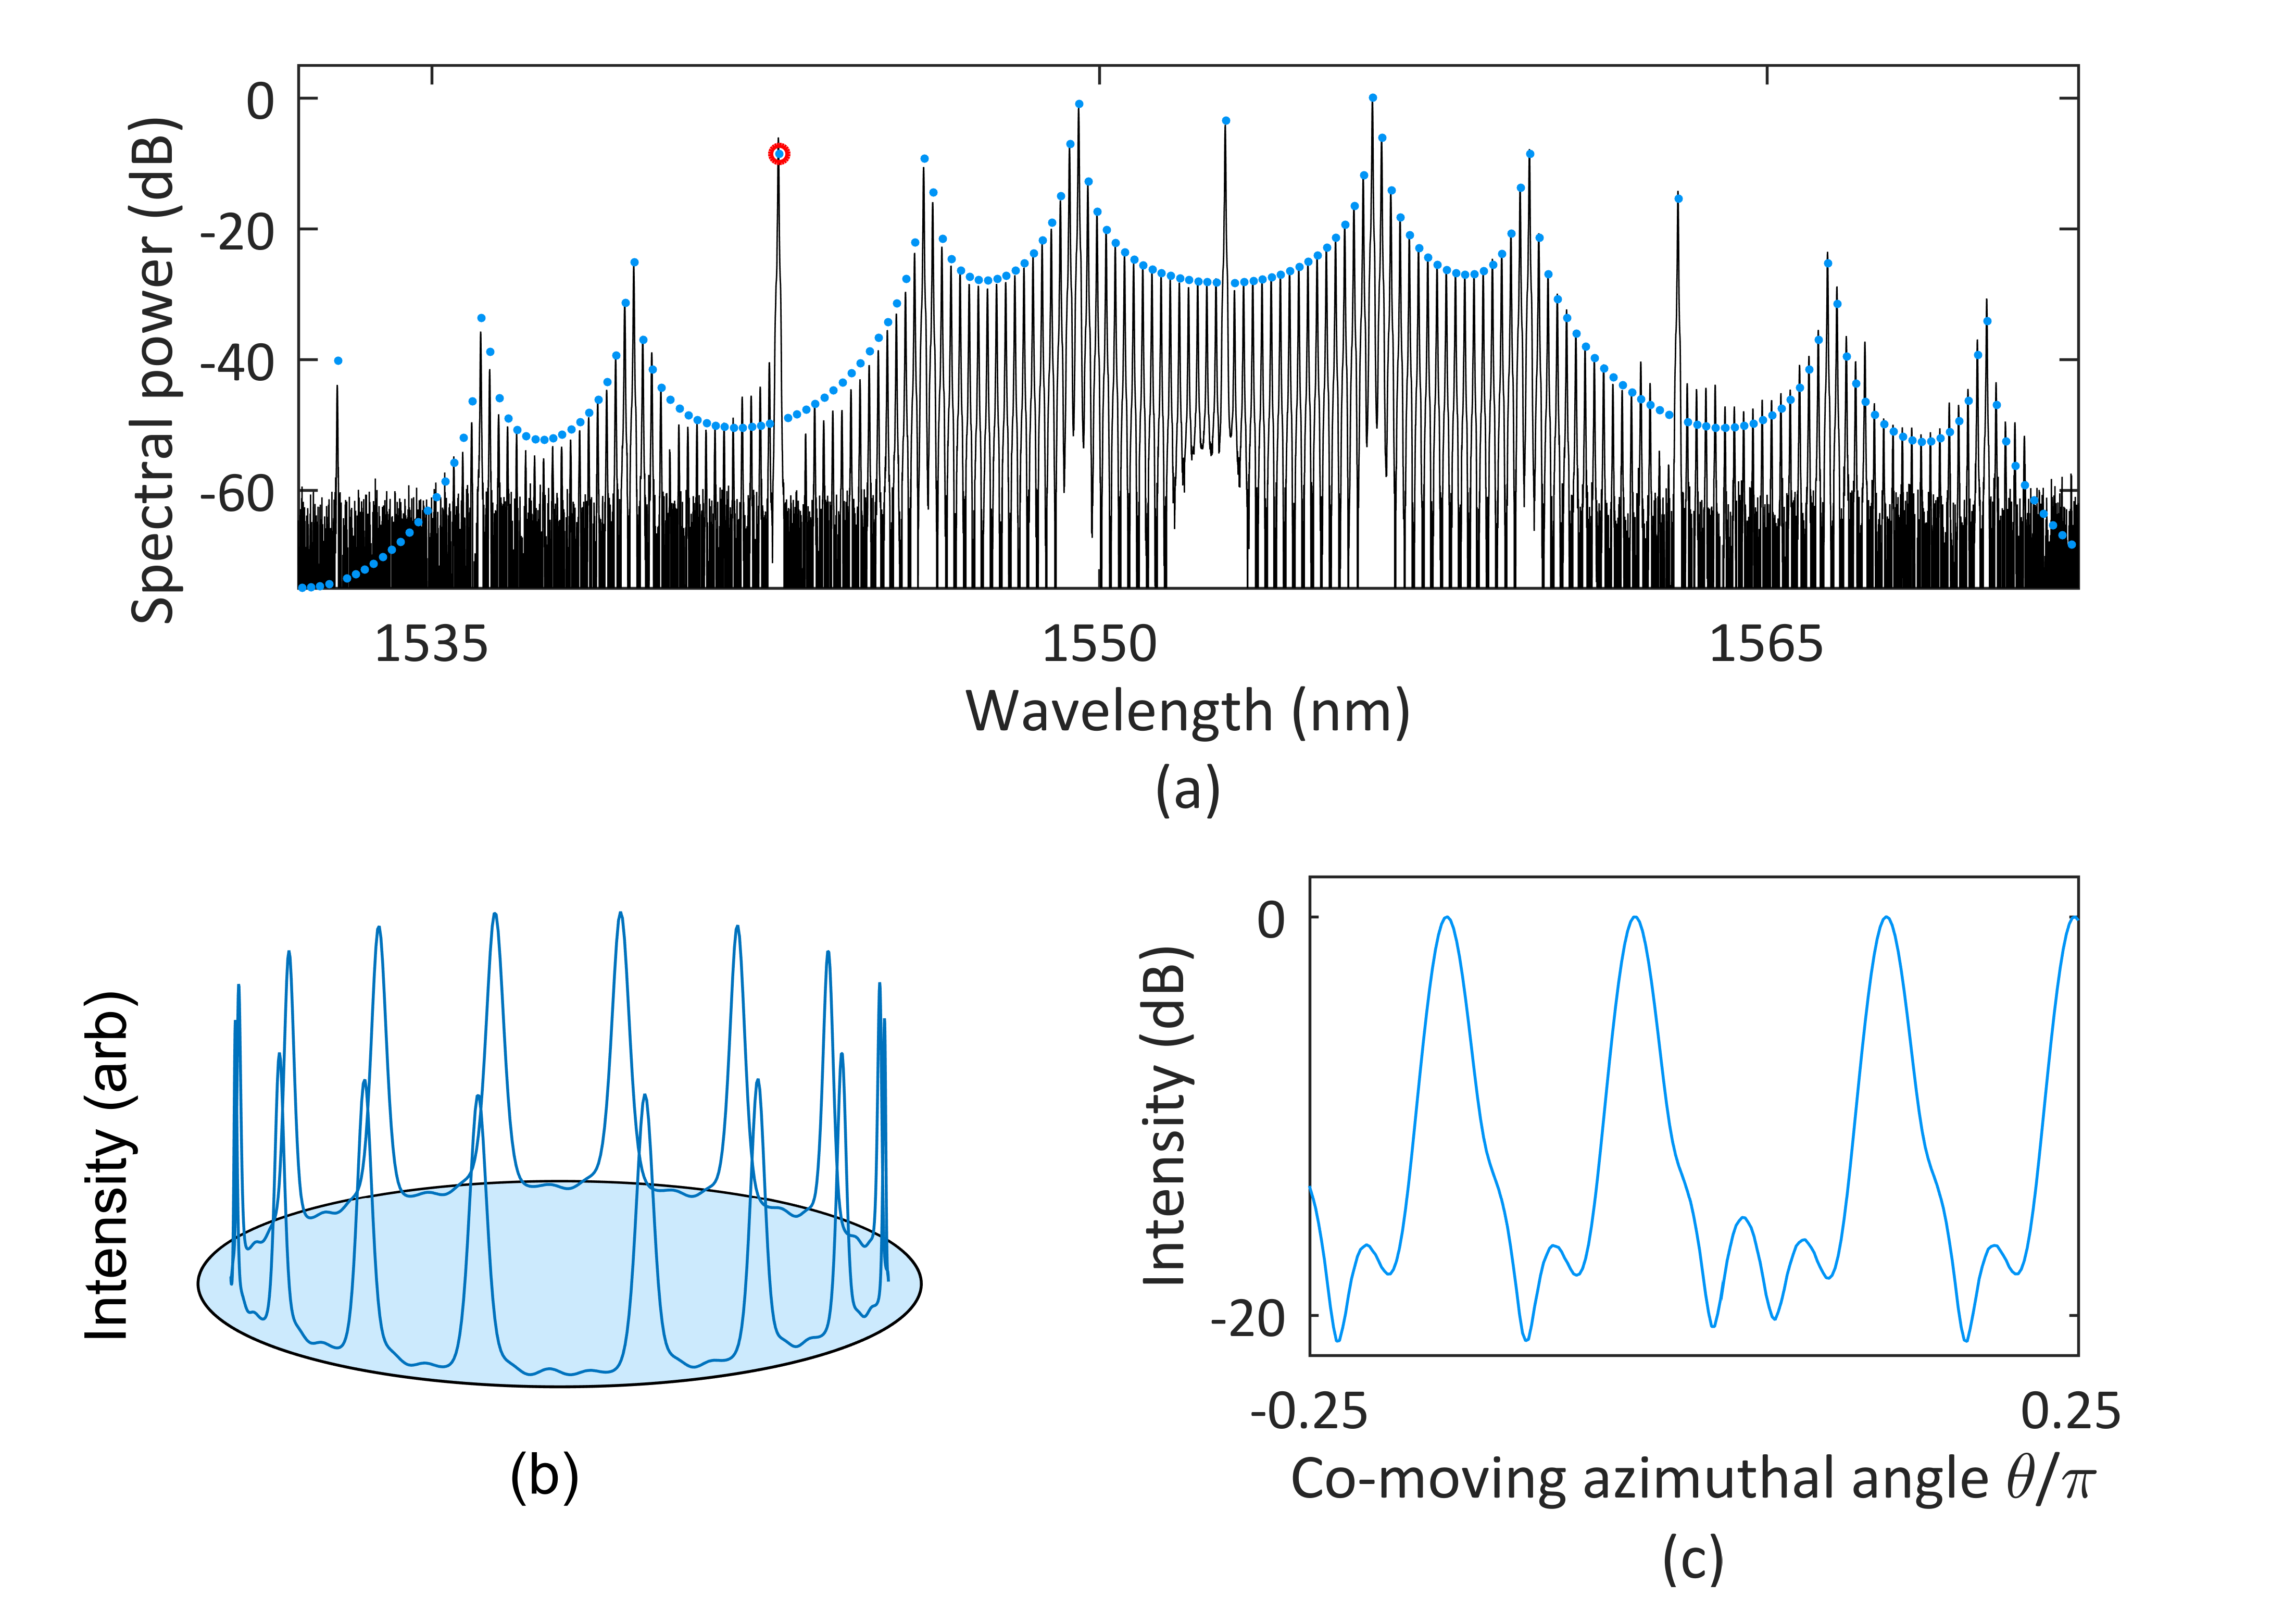
\includegraphics{\FigPath/Figures/SolitonCrystals/SCsuperstructure.png}
	\end{center}
	\caption[Figure Title]{\textbf{title}text}
	\label{fig:SCsuperstructure}
\end{figure} 

To gain insight into crystal generation, we simulate laser frequency scans across the resonance that generate this crystal in the presence of the mode crossing on mode 49. Example scans are shown for the case without the mode crossing (green) and with it (blue) in Fig. 2d. In both scans, solitons emerge from chaos as the frequency of the laser is decreased. In the presence of the mode crossing, they are generated with inter-soliton separations of $2\pi n/49$ radians. A greater number of solitons emerge from chaos in the presence of the mode crossing, and this higher number helps to stabilize the crystal against thermal changes in the experiment. Further, upon continuation of the simulation, some of the solitons in the scan without the mode crossing interact attractively and pair-annihilate, while the crystallized ensemble resulting from the scan with the mode crossing remains stable indefinitely.

\begin{figure}[htpb]
	\begin{center}
		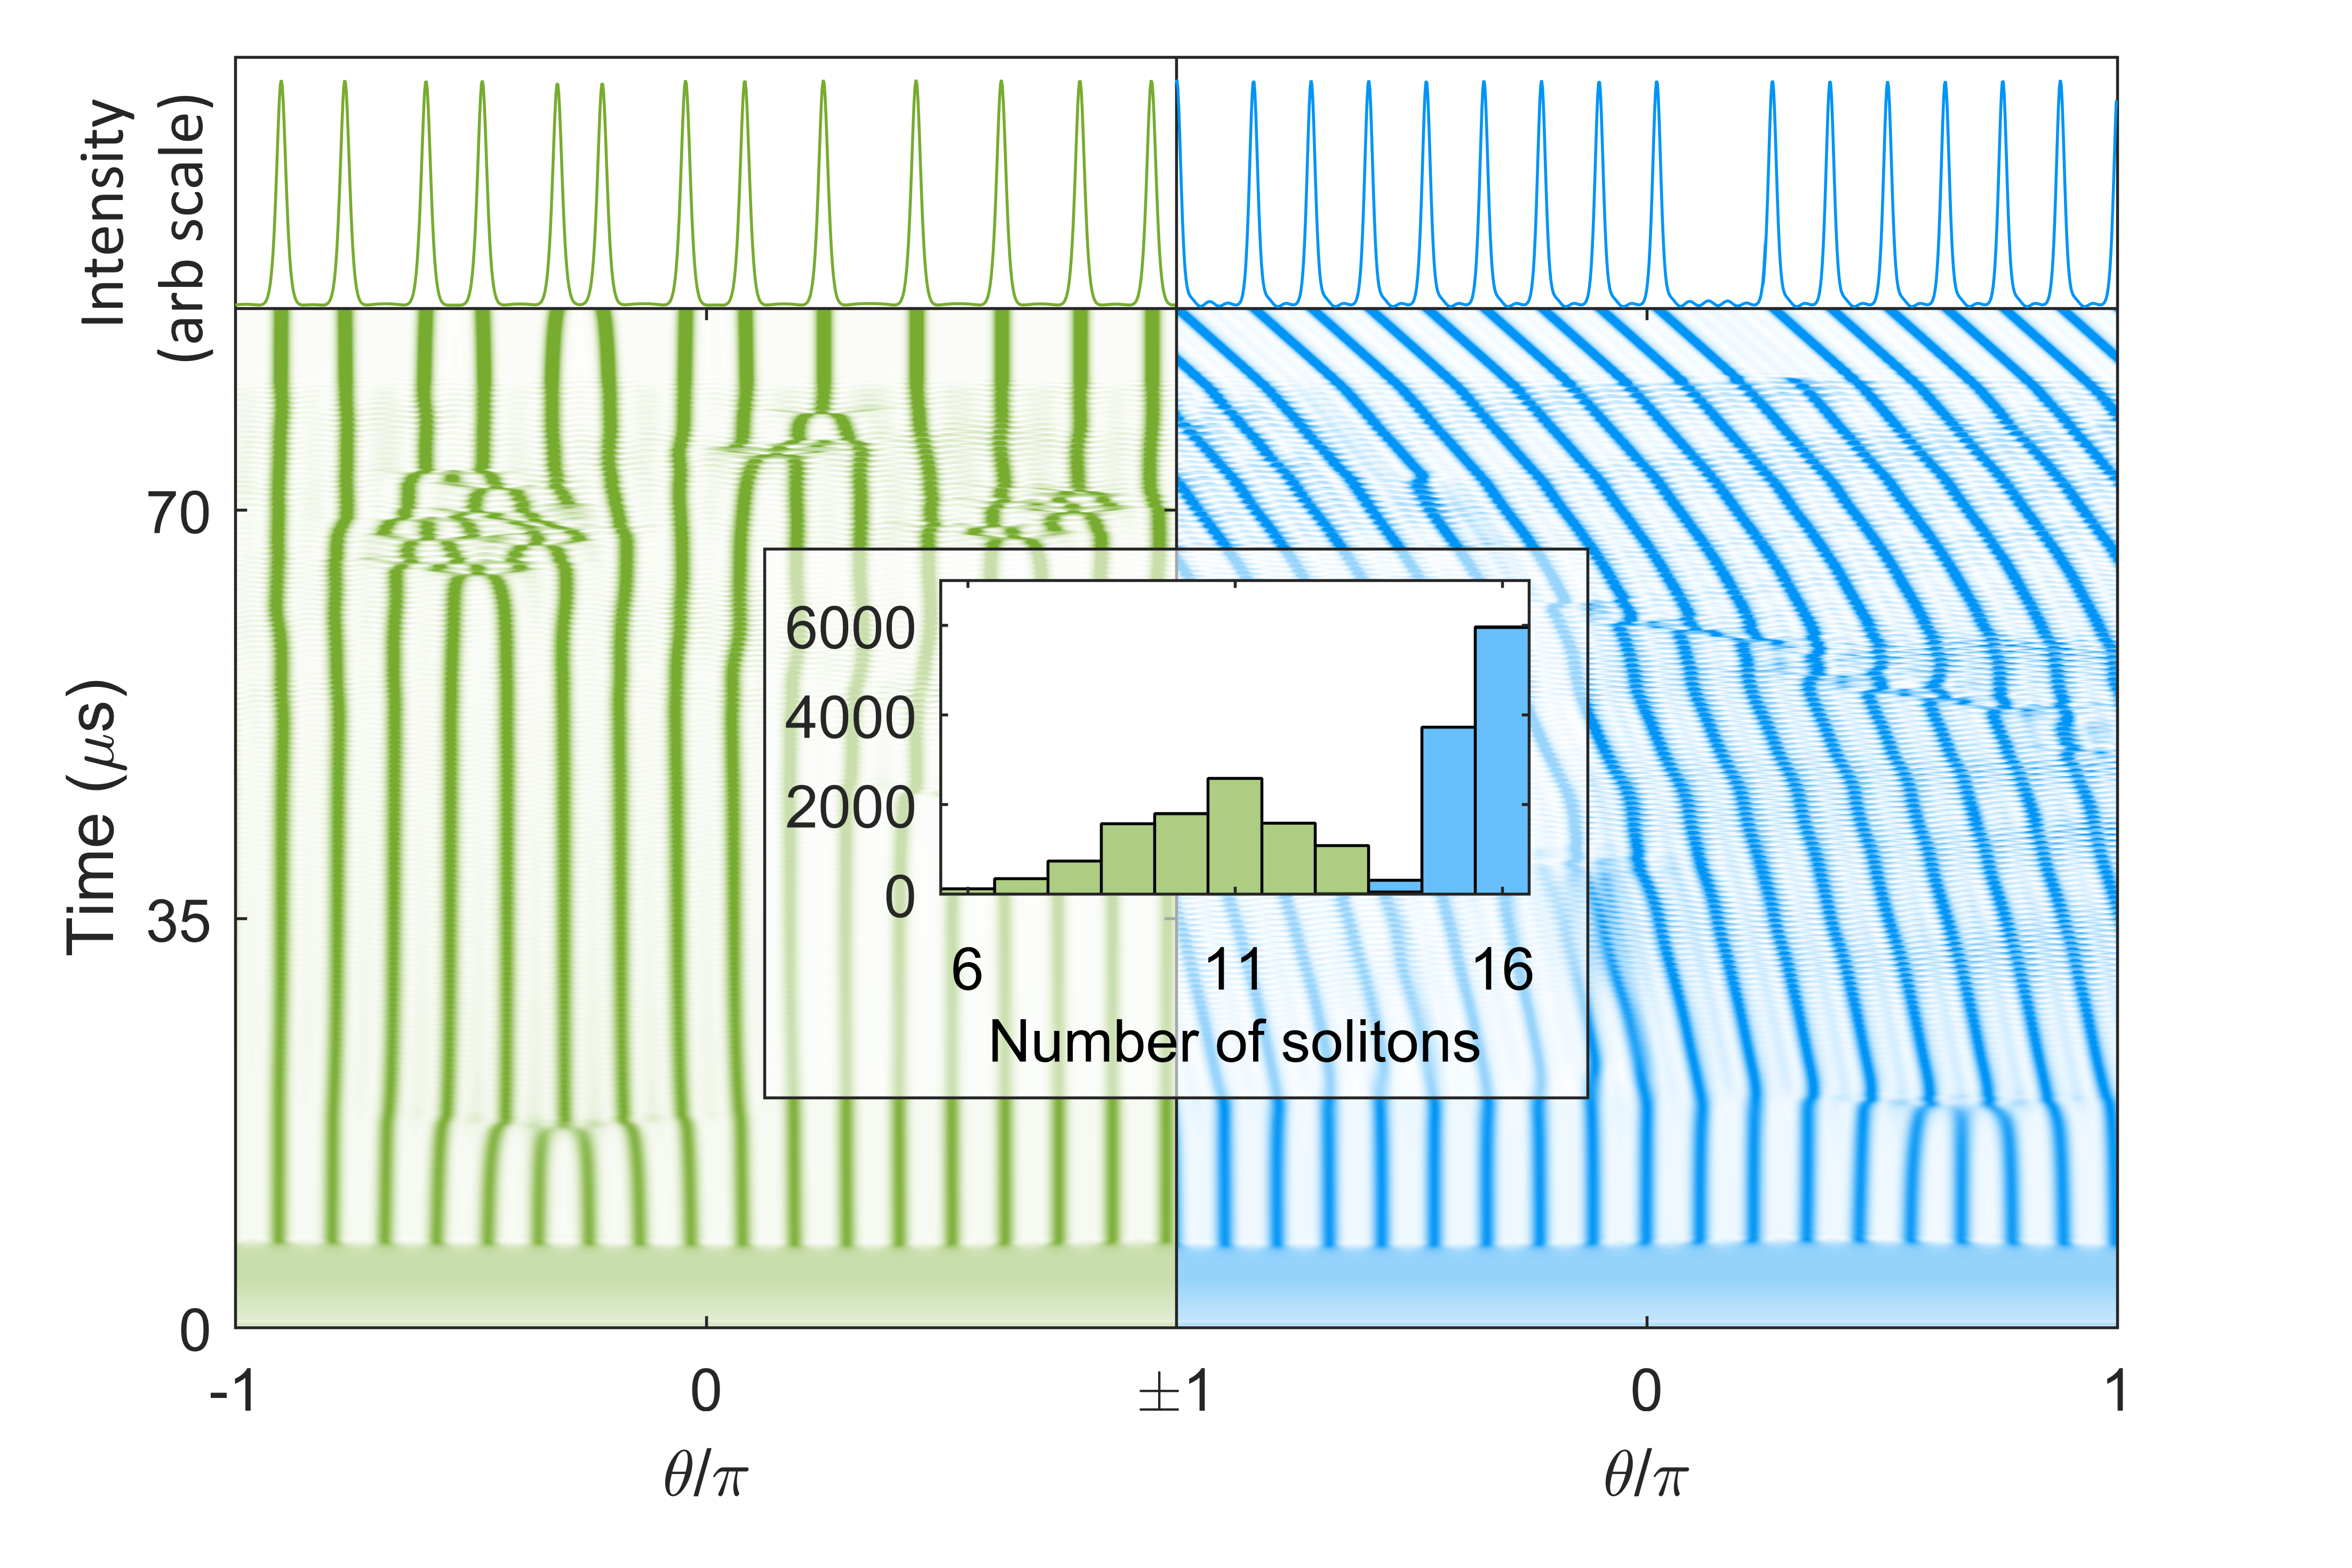
\includegraphics{\FigPath/Figures/SolitonCrystals/SCsimgen.png}
	\end{center}
	\caption[Figure Title]{\textbf{title}text}
	\label{fig:SCsimgen}
\end{figure} 

We investigate the pair-distribution function (PDF) for the soliton ensembles generated by these scans. The PDF is the probability that a soliton exists at position $\theta_0+\Delta\theta$ given that a different soliton exists at position $\theta_0$, normalized to the density. This is a useful metric to classify particle interactions which we borrow from condensed matter physics (see e.g. Ref. \cite{42}, especially Fig. 2, and Ref. 43, especially Fig. 1.1 and Chapter 3). We note that for numerically calculated discrete PDFs the absolute scaling of the PDF is not important, as it depends on the density of numerical sampling. In Fig. 2e, we plot the average PDFs for 10000 simulated scans with and without the mode crossing. The result for the case with a mode crossing is sharply peaked, indicating that the allowed inter-soliton separations take on discrete values. The result for the case without the mode crossing is continuous, with a peak near the most likely nearest-neighbour separation and periodic revivals at its multiples, falling to the value of the PDF for uncorrelated soliton positions (the density) at large separations. This is exactly the expected form of the PDF for a liquid \cite{42,43}. For comparison, we plot a PDF (black, Fig. 2e) generated by simulation of a simple particle ensemble with mean inter-particle separation of $\Delta\theta=0.155\pi$ and normally distributed noise on this value with standard deviation of $\sigma_{\delta\theta}=0.18\Delta\theta$. Thus, with a particle labelled by $n = 0$ fixed at $\theta = 0$, the position of particle $n$ is $\theta_0 = n\Delta\theta + \Sigma_n\delta\theta_i$, with $\delta\theta_i$ the instantiations of the random variable representing the noise on the pulse spacings. 

\begin{figure}[htpb]
	\begin{center}
		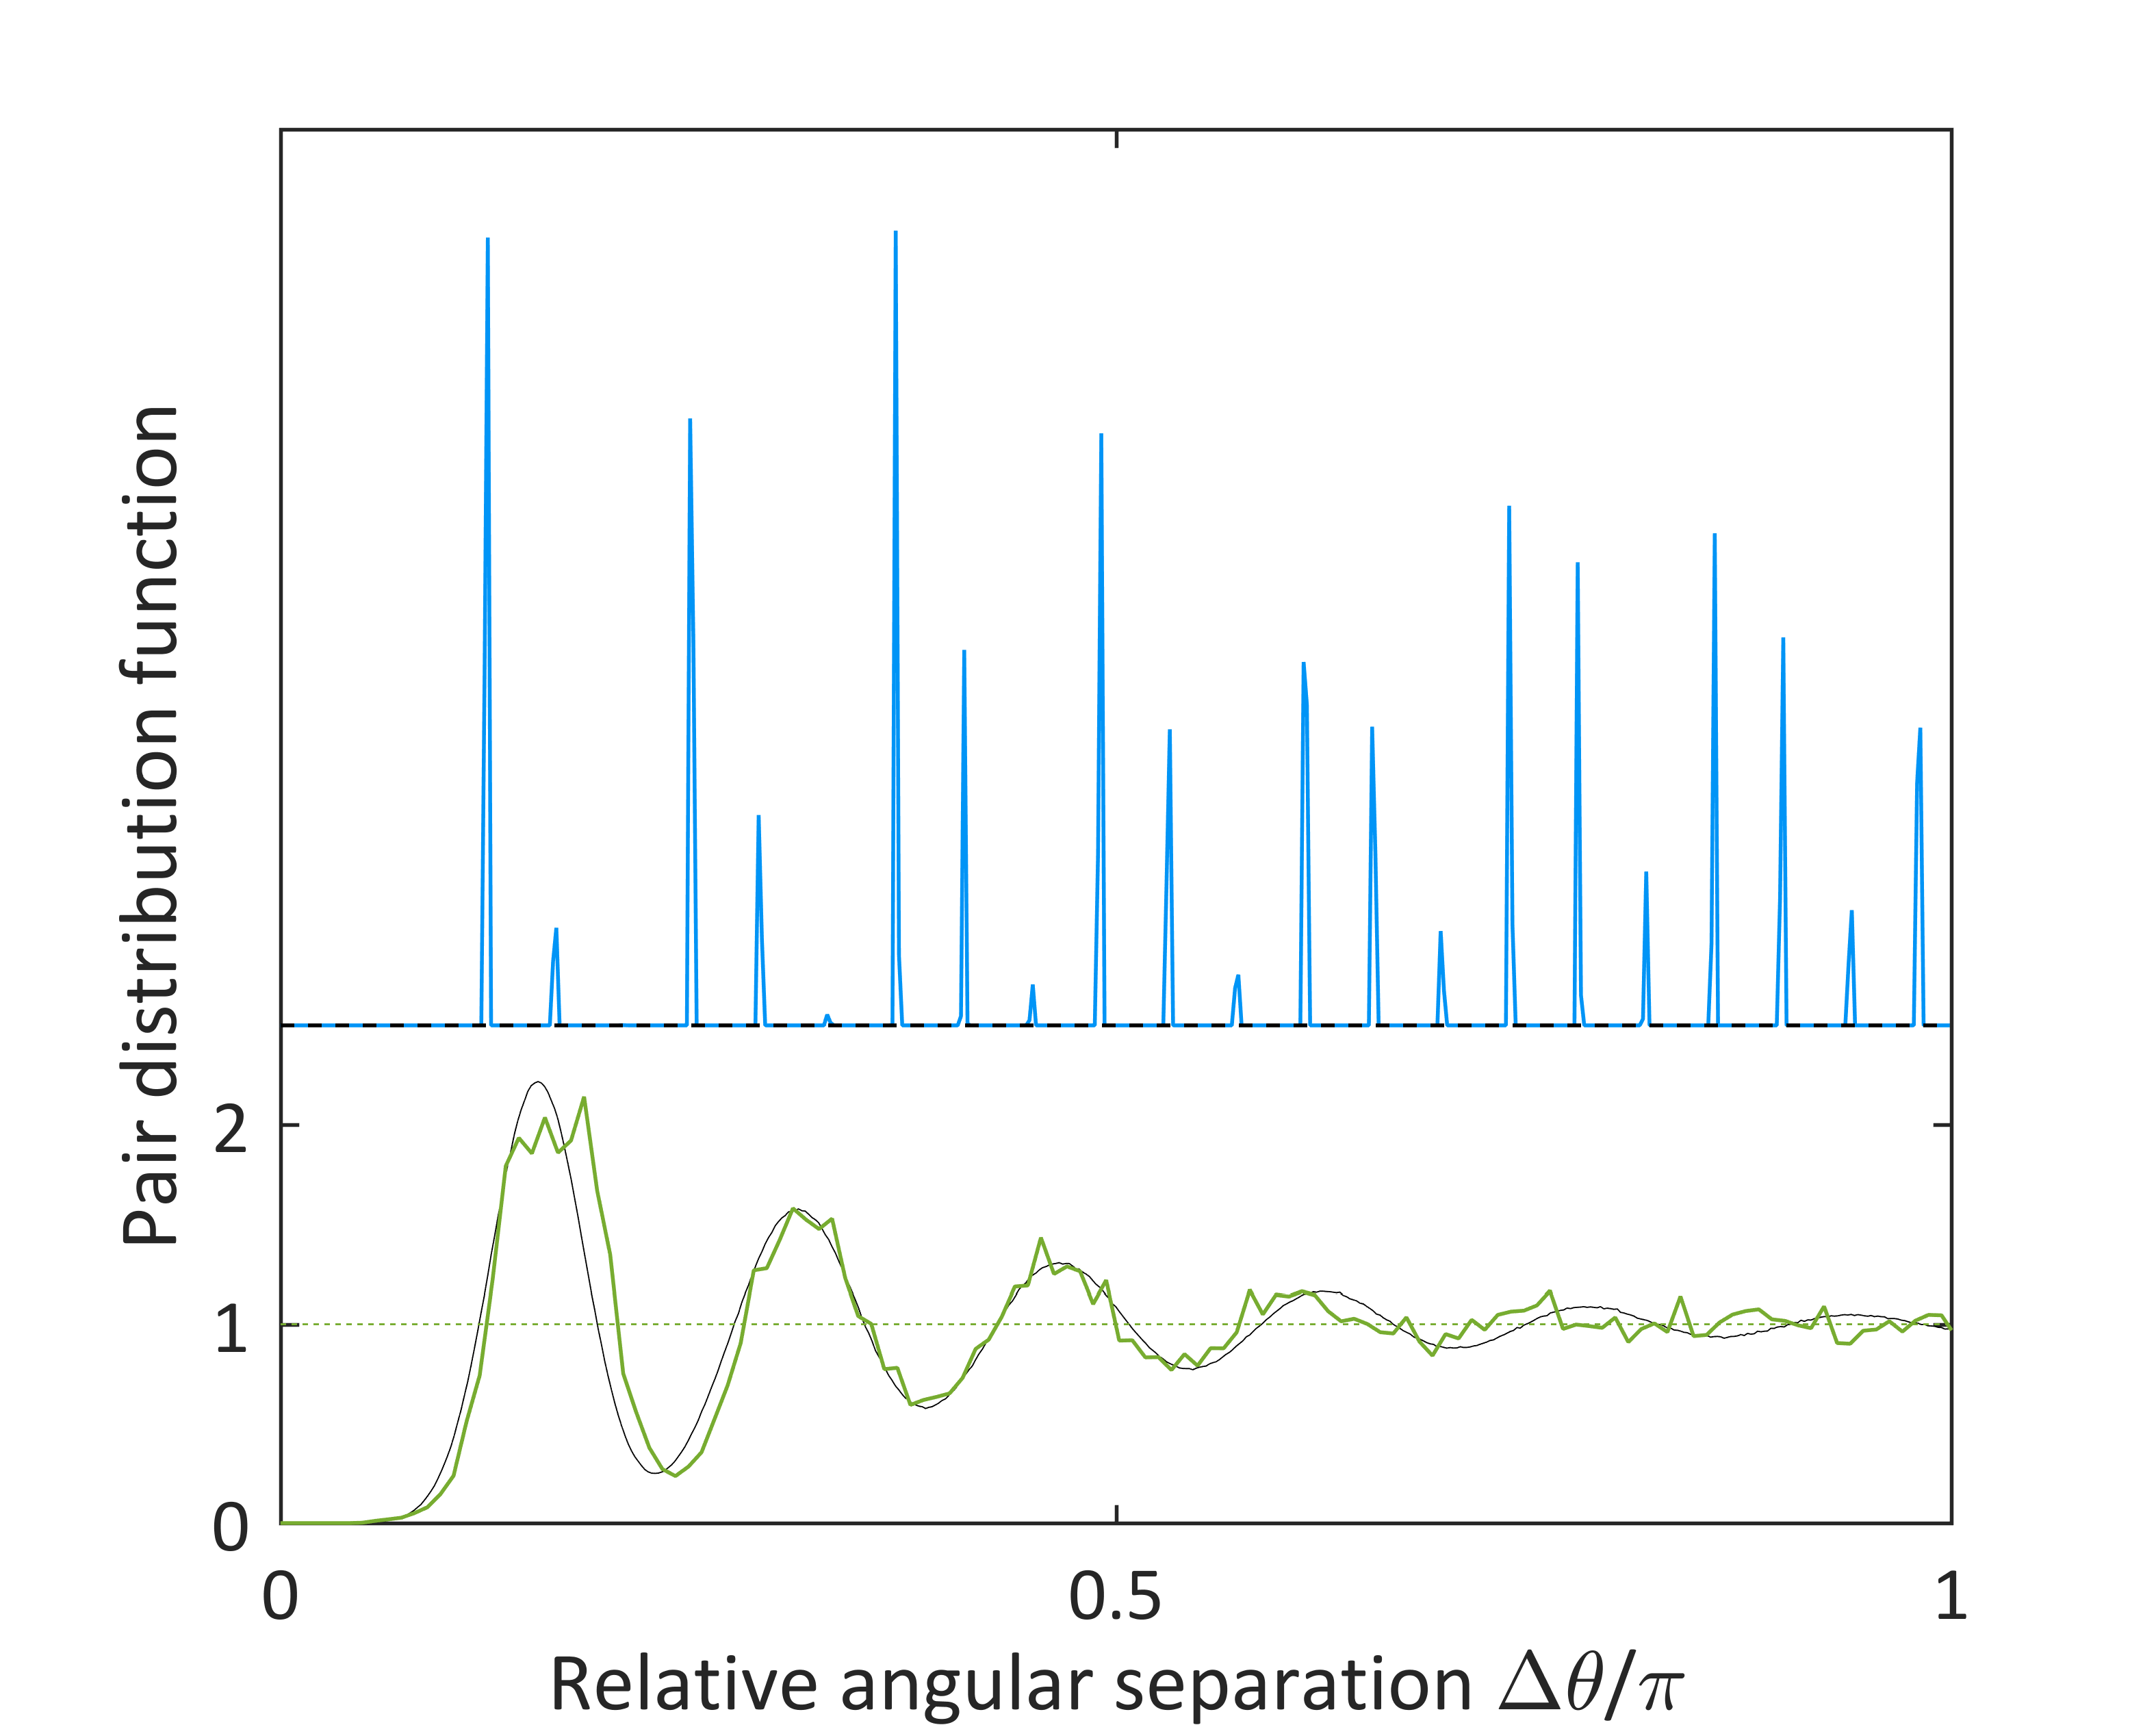
\includegraphics{\FigPath/Figures/SolitonCrystals/SCpdf.png}
	\end{center}
	\caption[Figure Title]{\textbf{title}text}
	\label{fig:SCpdf}
\end{figure} 


 
\section{Soliton crystal configuration space}\label{SCtaxonomy}

We observe a rich variety of soliton crystals explained by ordering in accordance with an extended background wave as described above; many of the optical spectra are plotted in Fig. 3. Operationally, we adjust the pump laser power to provide repeatable conditions for creating particular crystals; more complex crystals occur with increased laser power, which intensifies the fluctuations in the chaos that precedes crystal generation and provides less well-ordered initial conditions. Once a crystal is generated, it is stable to small adjustments in the pump power and detuning, as the crystal structure is determined by the initial conditions for soliton formation rather than by an explicit dependence on pump power or detuning. The crystals we observe exhibit vacancies (Schottky defects)\cite{27}, Frenkel defects\cite{27}, disorder, or superstructure, or some combination thereof. A Frenkel defect consists of the shifting of a soliton in an otherwise uniform crystal. Disordered crystals are crystals in which the solitons fall on the peaks of the extended background wave, but their distribution across these peaks varies without any apparent regular order or favoured period. 

We highlight the crystal plotted in Fig. 3n. This crystal exhibits both superstructure, with a superlattice period of $2\pi/3$ radians, and a Frenkel defect. Three identical supercells per resonator round-trip yield a spectrum which has light in optical modes spaced by three resonator FSR, because the waveform’s period has been reduced threefold. The Frenkel defect, occurring once per round-trip, contributes the single-FSR lobes to the spectrum. The result is three bursts of 8, 9, and 10 solitons respectively. 	

Fig. 3o shows a soliton crystal with inter-soliton separations that are slightly irregular and which we have not simulated as a steady-state solution of any perturbed LLE. We expect that the formation of the crystal and the distribution of solitons are dictated by mode interactions, but that in this case our simple approximation of a perturbation to the LLE by a reduced comb-resonator detuning on a single comb mode is not appropriate.
Finally, we highlight the series of crystals plotted in Figs. 3p-3t. This series of crystals was generated by moving the pump laser closer to a mode-crossing in steps of integer multiples of the resonator FSR. This data demonstrates the influence of the background beating between the pump laser and the mode-crossing in determining the configuration of solitons in the resonator.


\begin{sidewaysfigure}[htpb]
	\begin{center}
		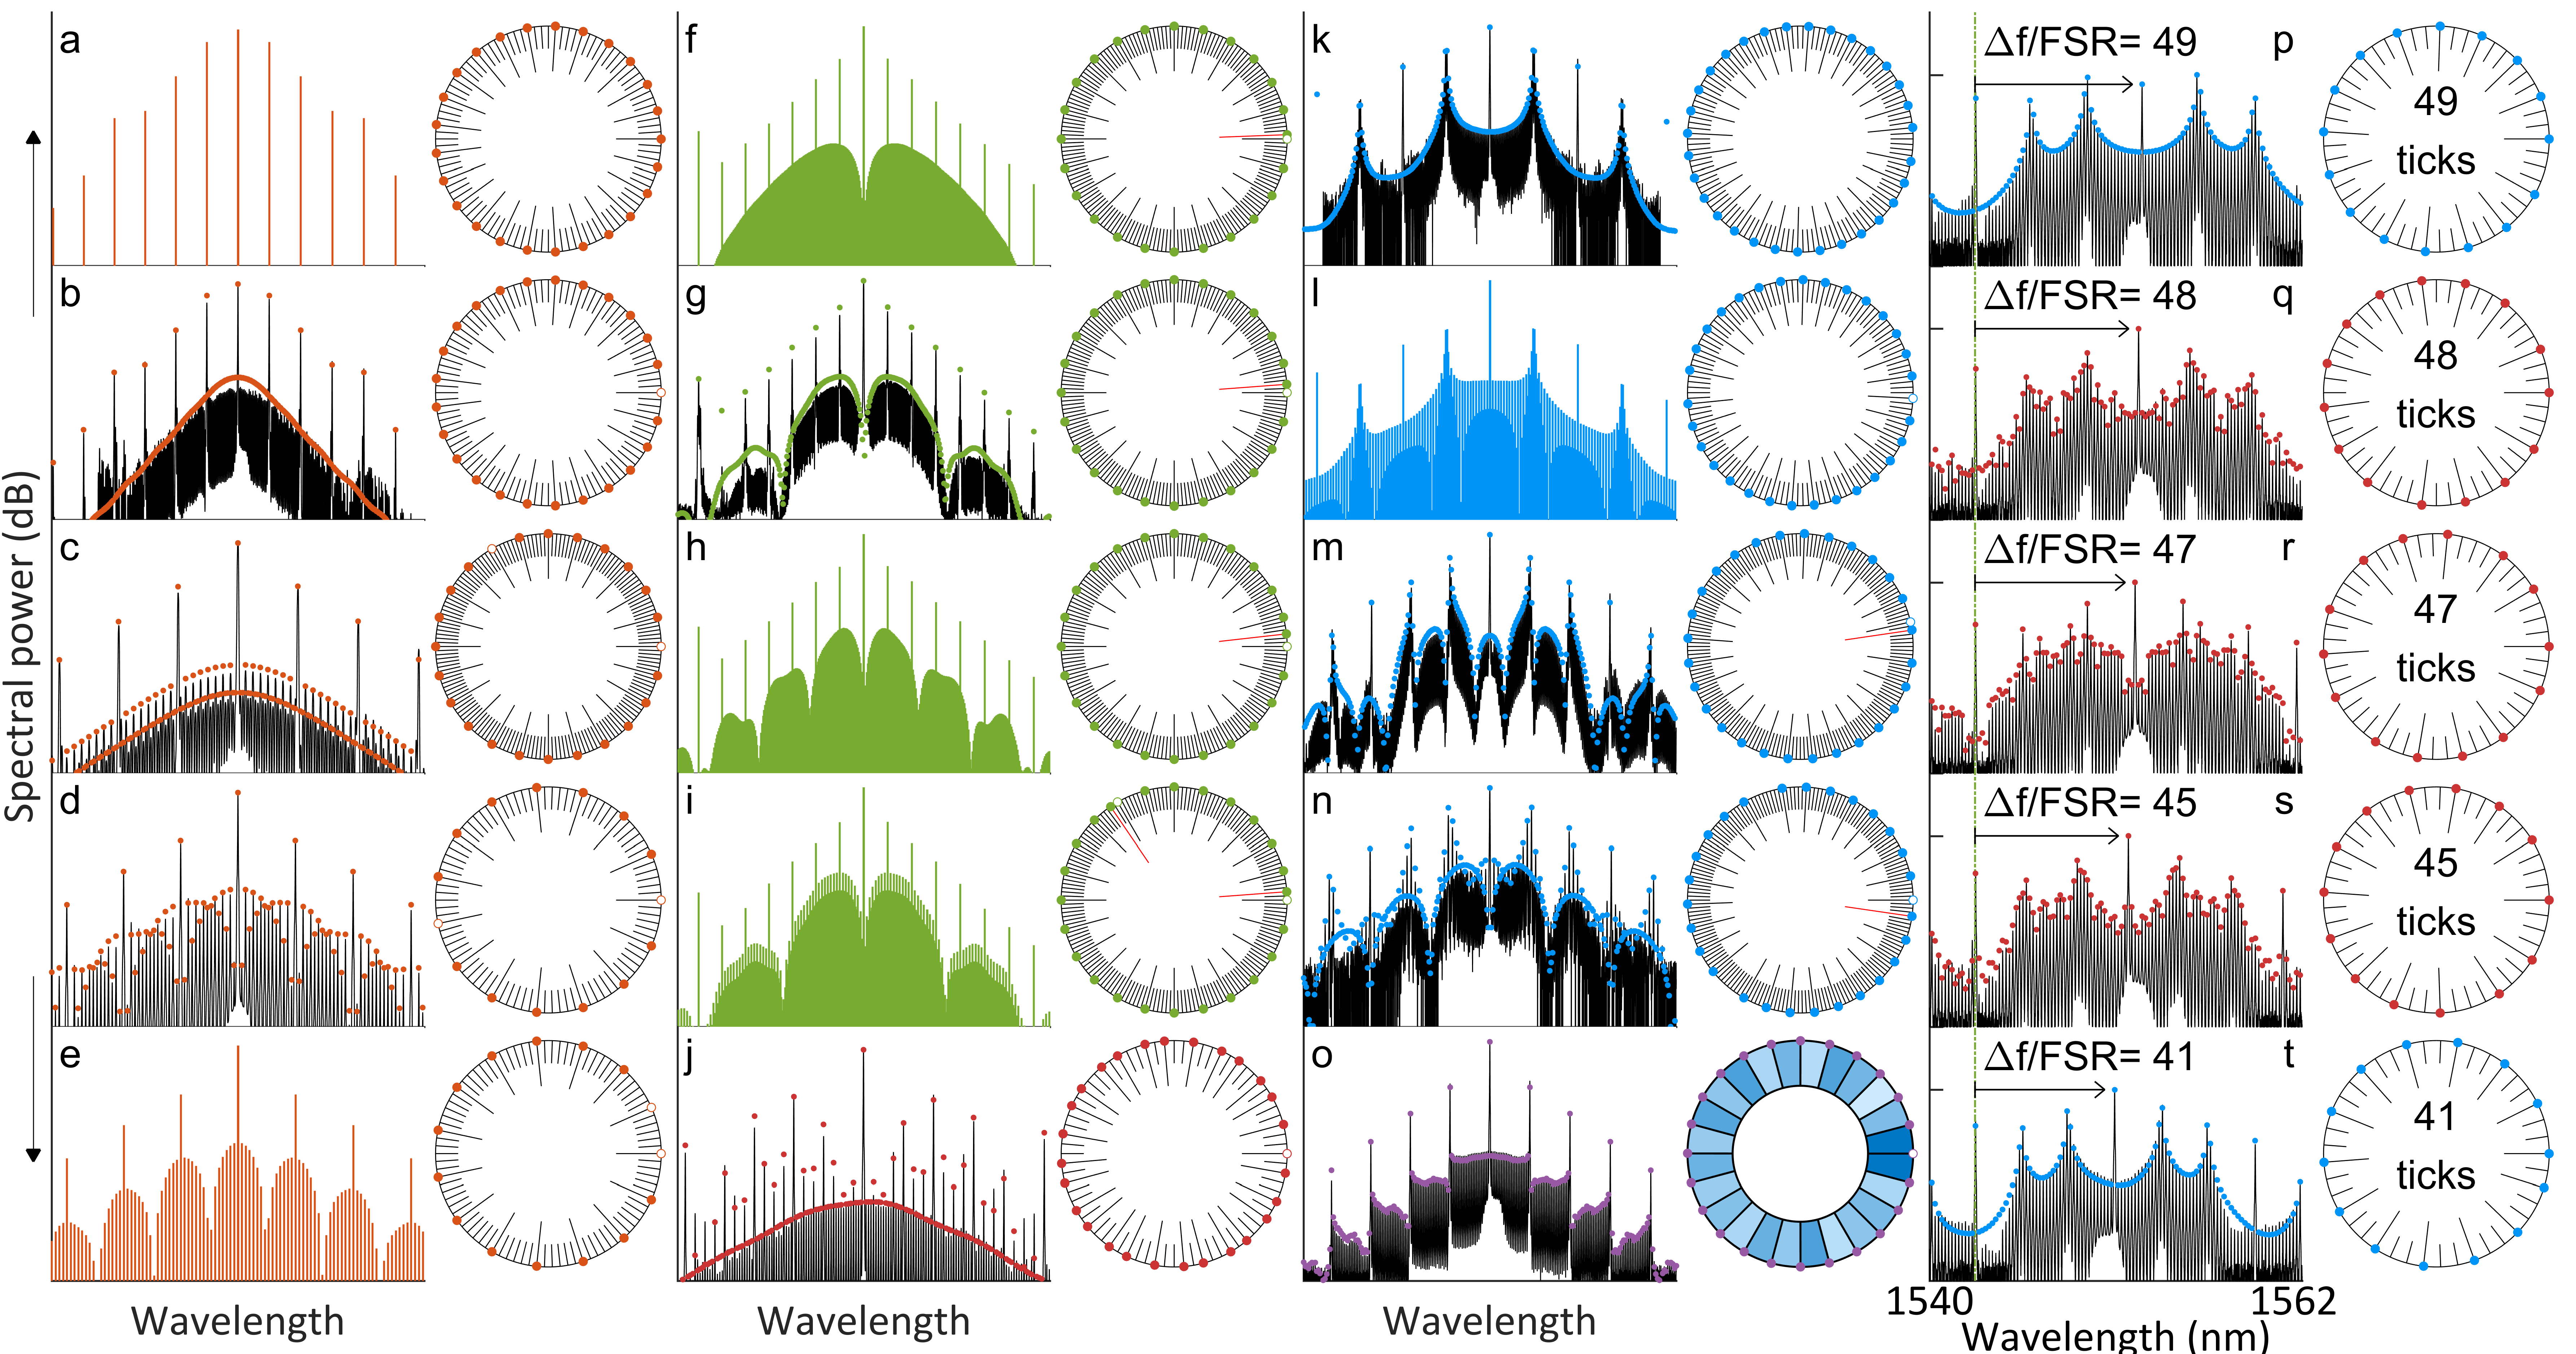
\includegraphics{\FigPath/Figures/SolitonCrystals/SCtaxonomy.png}
	\end{center}
	\caption[Figure Title]{\textbf{title}text}
	\label{fig:SCtaxonomy}
\end{sidewaysfigure}




